\chapter{Serviços críticos}
\label{cap:servicoscriticos}

No capítulo anterior foram detalhados os serviços que estão disponíveis na empresa. Neste capítulo serão apresentados os serviços 
que foram considerados críticos para a empresa, sendo que para a definição desses foram adotados alguns critérios. Esses critérios foram criados
através de uma análise dos serviços, levando em consideração a importância para a empresa, para o seu ambiente e a opinião da direção da empresa
%da mesma forma que o autor \citet{geordano2014} definiu a relevância de seus critérios.
\cite{geordano2014}. Mais especificamente, os critérios definidos foram:

%Para a definição desses critérios utilizou-se uma metodologia semelhante à utilizada no artigo de \citet{geordano2014}. O autor 
%comparou ferramentas para monitoramento de redes de fibra óptica, para isso, ele criou critérios baseados na tecnologia foco do trabalho 
%(tecnologia PON), além de levar em consideração desempenho e \ac{SLA}. Para a definição da relevância de cada critério, o autor considerou
%a importância do critério para o ambiente monitorado da empresa e também a opinião da direção da empresa.
%tcc geordano - bom tempo, orientador maria de fatima, Monitoramento_snmp_redes_Geordano_Arend.pdf

\begin{itemize}
 \item A quantidade de clientes que utilizam o serviço: esse é o critério mais relevante, pois impacta diretamente no faturamento
 da empresa. De fato, se um cliente ficar sem acesso à Internet, o cliente terá um desconto proporcional ao tempo que ficou sem 
 acesso; 
 \item O número de requisições: esse número é importante, uma vez que, indica a quantidade de usuários que dependem do serviço e a frequência
 de utilização do serviço. Esse critério engloba, por exemplo, o número de conexões \aca{TCP}, o número de requisições 
 \aca{UDP}, a quantidade de acessos em um servidor de hospedagens de sites e a quantidade de requisições \aca{DNS} 
 em um servidor recursivo;
 %\aca{TCP} \cite{tanenbaum2011}, \aca{UDP} \cite{tanenbaum2011}
 \item O volume de elementos do serviço: essa medida demonstra a abrangência do serviço, ou seja, quantos clientes são dependentes deste. 
 Como exemplo de elementos pode-se citar a quantidade de contas de \textit{e-mail} ativas em um servidor de \textit{e-mail} ou a quantidade de 
 equipamentos monitorados por um servidor.
 %Esse critério é importante pois com ele pode-se comparar diferentes serviços possibilitando perceber o grau de relevância que cada um possui;
 %Esse critério, como o anterior, também permite comparar diferentes serviços para ter a possibilidade de ordená-los de acordo com sua relevância, 
 %por isso o torna importante para esta análise.
\end{itemize}

Nas próximas seções serão descritos os serviços que foram considerados críticos, com base nos critérios apresentados.

\section{DNS recursivo primário}
\label{section:dnsrecprim}

Esse serviço foi classificado como o serviço mais importante pois possui um impacto direto nos clientes do provedor. Além disso, esse é o único 
serviço que todos os clientes e funcionários utilizam, totalizando aproximadamente 9000 pessoas. O objetivo de um provedor é fornecer uma navegação 
de qualidade aos seus clientes, sendo assim, o \ac{DNS} é fundamental para essa navegação. A importância deste serviço está ilustrada na Figura 
\ref{fig:dns_udp} (a), onde pode ser observado que esse serviço possui picos de aproximadamente 1150 requisições por segundo. Já na Figura 
\ref{fig:dns_udp} (b) pode ser observado que o servidor \textit{Passata} é o servidor que apresenta o maior número de requisições 
\ac{UDP}\footnote[1]{Esse número de requisições \ac{UDP} é elevado devido ao fato do serviço \ac{DNS} utilizar esse protocolo de transporte.}. 
Essa figura compara os principais servidores da empresa através de requisições \ac{UDP} e pode ser usada como um indicador da quantidade de 
clientes que utilizam determinados serviços.

\begin{figure}[h!]
 \centering
 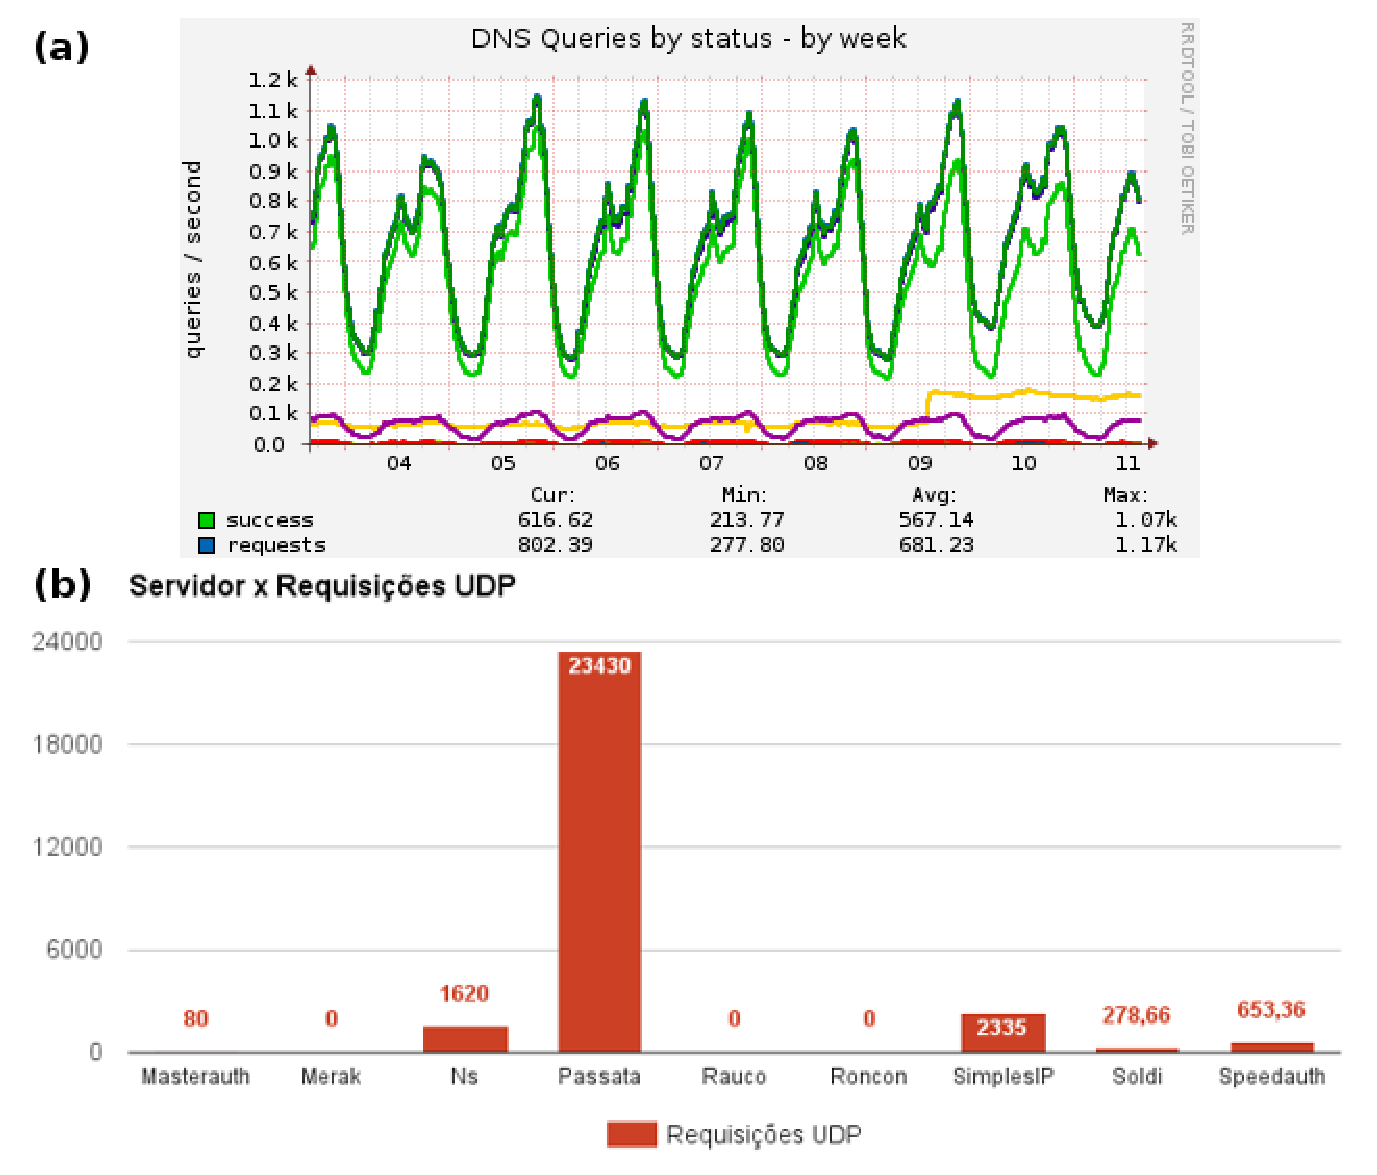
\includegraphics[width=400px]{img/dns_udp.eps}
 \caption{Gráfico de requisições DNS por segundo do período de uma semana (a) e comparação de requisições UDP simultâneas máximas entre 
 os principais servidores (b).}
 \label{fig:dns_udp}
\end{figure}

\section{Autenticação Radius}
\label{section:radius}

Esse serviço é importante pois é o responsável pela autenticação de todos os clientes do provedor. Caso esse serviço fique indisponível, 
os clientes não conseguirão estabelecer conexão e, consequentemente, não conseguirão utilizar o serviço de Internet. Os servidores 
\textit{Masterauth} e \textit{Speedauth} fornecem o serviço de \textit{Radius}, sendo que esses recebem em média, 1,6 requisições de autenticação 
por segundo. Além disso, esses servidores armazenam dados relacionados à conexão dos clientes, como por exemplo, o endereço de \ac{IP} que é 
utilizado por um cliente em um determinado período de tempo, o tráfego de dados da conexão, o tempo de conexão, o endereço \aca{MAC} dos 
equipamentos dos clientes, entre outros. Essas operações resultam em média 23 requisições por segundo. 
Outro critério que é relevante para esses servidores é o volume de elementos do serviço, que neste caso, representa a quantidade de clientes que
utilizam esses servidores para autenticação. De fato, como pode-se observar na Figura \ref{fig:elementos_tcp} (a) que os servidores 
\textit{Masterauth} e \textit{Speedauth} estão entre os que apresentam um maior número de contas. Além disso, nesses servidores existe um grande 
número de conexões \ac{TCP}\footnote[1]{Esse número de conexões \ac{TCP} deve-se ao fato do \textit{software} \textit{Freeradius} utilizar esse 
protocolo para a comunicação com o seu banco de dados.} simultâneas, como pode ser observado na Figura \ref{fig:elementos_tcp} (b).

% \begin{figure}[h!]
%  \centering
%  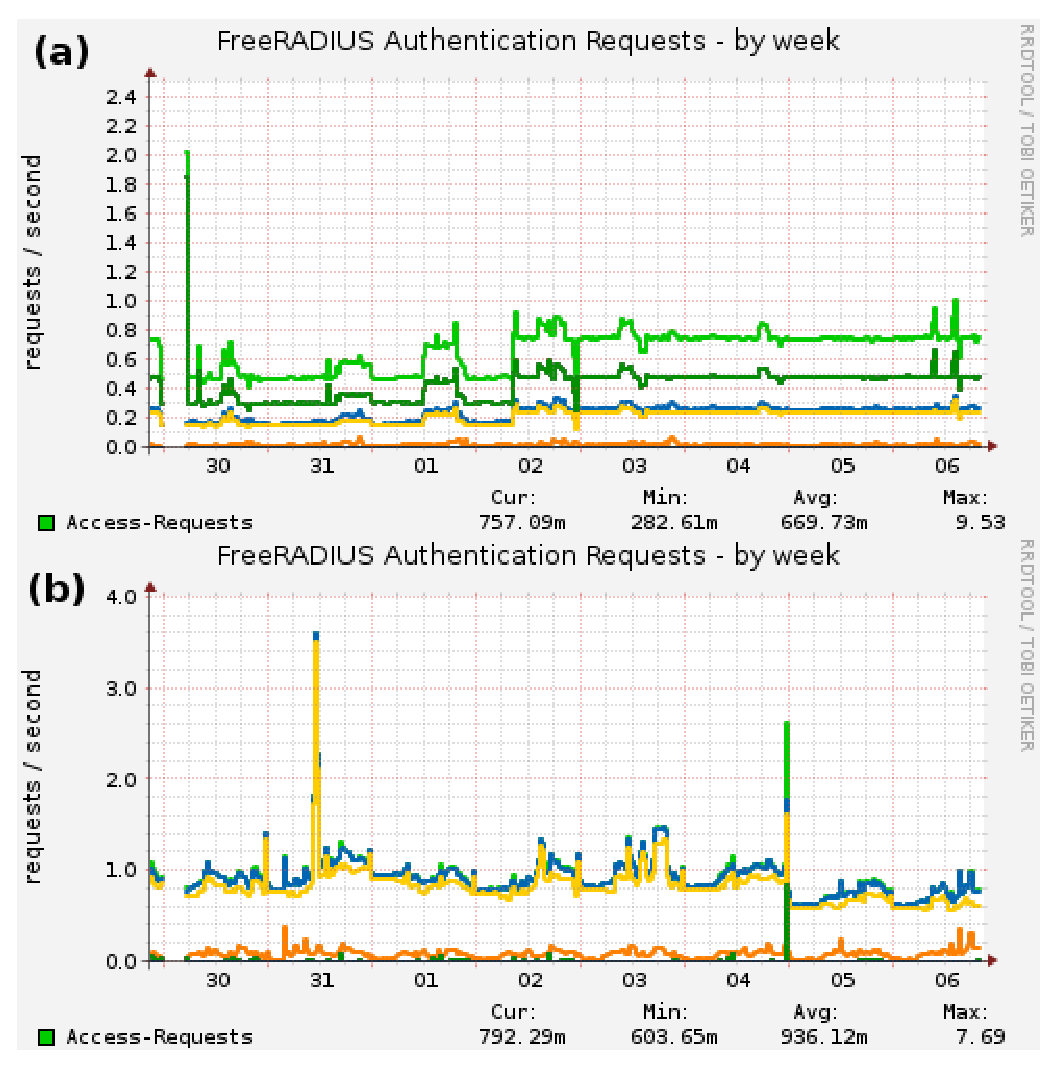
\includegraphics[width=300px]{img/freeradius_auth.eps}
%  \caption{Gráfico de requisições de autenticação do servidor \textit{Masterauth} (a) e \textit{Speedauth} (b).}
%  \label{fig:freeradius_auth}
% \end{figure}

\begin{figure}[h!]
 \centering
 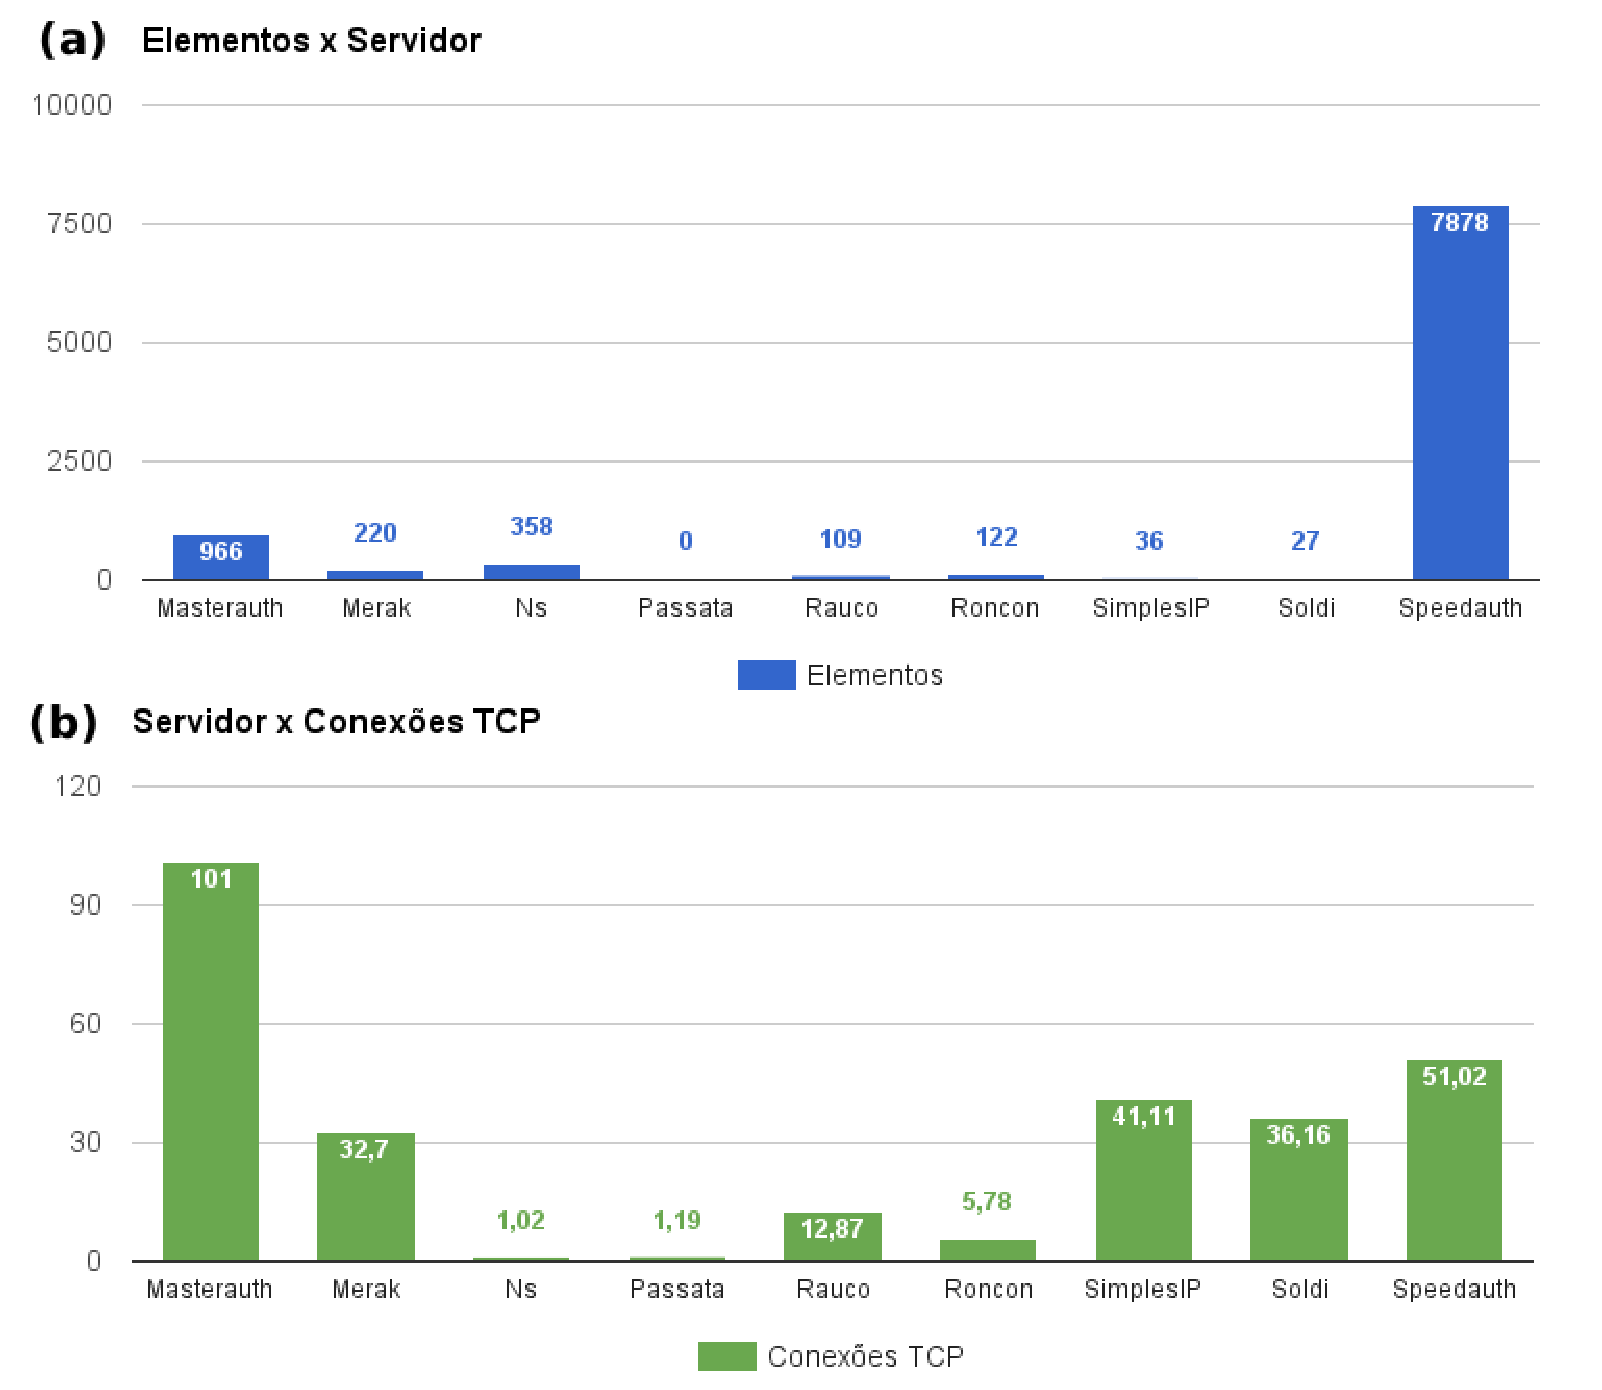
\includegraphics[width=380px]{img/elementos_tcp.eps}
 \caption{Gráfico de comparação de elementos (a) e de conexões TCP simultâneas máximas (b) entre os principais servidores.}
 \label{fig:elementos_tcp}
\end{figure}

\section{Sistemas da empresa e do provedor}
\label{section:sistemas}

O sistema do provedor é responsável pela maior parte das operações gerenciais do provedor. Este sistema é responsável pela emissão de 
boletos, atendimento de clientes, comunicação interna da empresa, vendas, ativações de novos clientes, entre outros. Esse sistema não tem um 
impacto direto para os clientes, porém é fundamental para o funcionamento da empresa e do provedor. Caso haja uma indisponibilidade desses sistemas 
a maior parte dos funcionários ficarão impossibilitados de trabalhar, sendo que a empresa possui um total de 65 funcionários.
%, sendo que são aproximadamente 35 funcionários simultâneos (de acordo com a Figura \ref{fig:ejabberd_week}), isso poderia gerar um prejuízo elevado para a empresa e o provedor. 

O sistema do provedor é executado no servidor \textit{Soldi} que recebe aproximadamente 3 requisições \aca{HTTP} por segundo
(Figura \ref{fig:soldi_week}). Além disso, a empresa mantém 28 sistemas de outros clientes nesse servidor. 
Como pode ser observado na Figura \ref{fig:elementos_tcp} (b), esse servidor encontra-se entre os que apresentam um maior número de conexões 
\ac{TCP}\footnote[1]{O número de conexões \ac{TCP} é considerado devido ao fato do protocolo \ac{HTTP} utilizar esse 
protocolo de transporte.}.
%\aca{HTTP} \cite{tanenbaum2011}

%\begin{figure}[h!]
% \centering
% 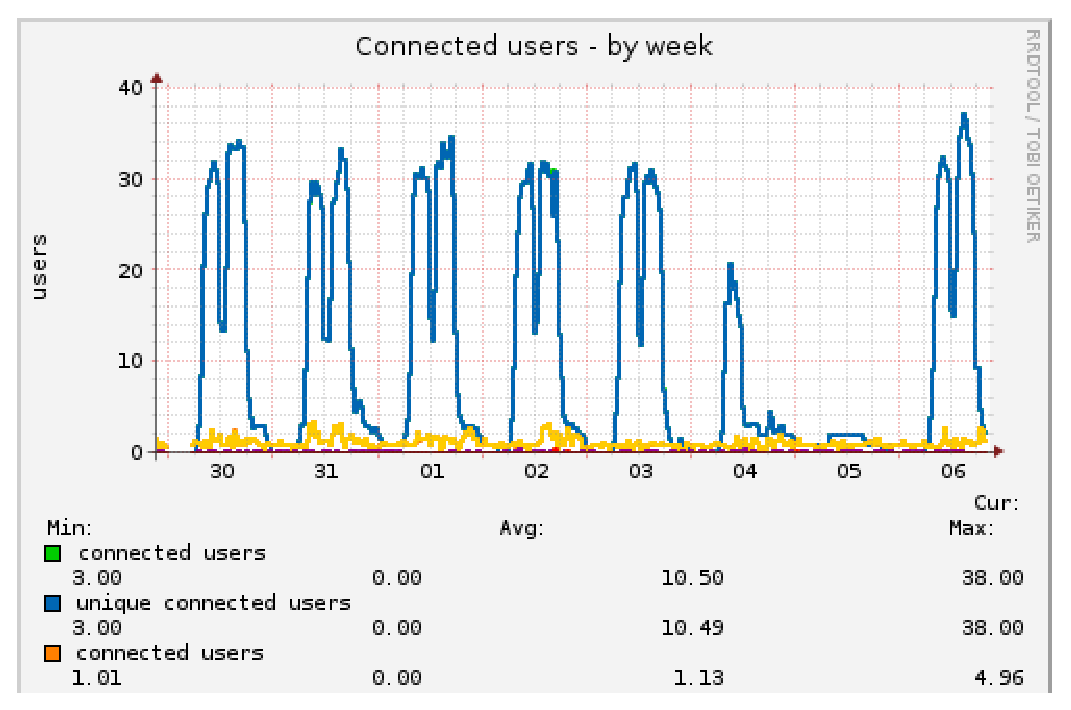
\includegraphics[width=310px]{img/ejabberd_week.eps}
% \caption{Gráfico usuários simultâneos de sistema.}
% \label{fig:ejabberd_week}
%\end{figure}

\begin{figure}[h!]
 \centering
 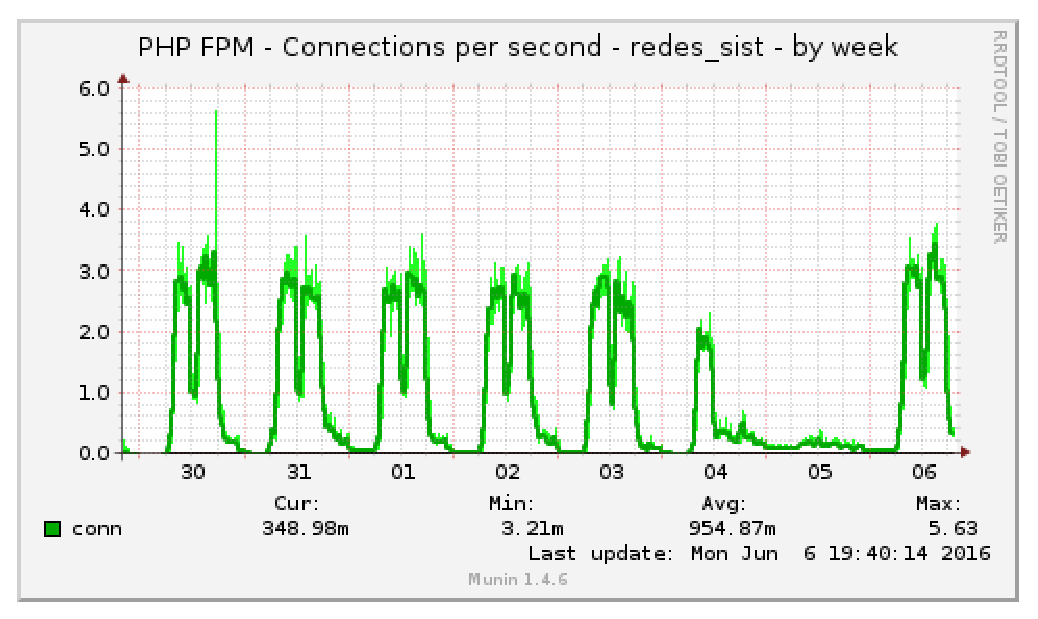
\includegraphics[width=280px]{img/soldi_week.eps}
 \caption{Gráfico de requisições por segundo do sistema do provedor durante o período de uma semana.}
 \label{fig:soldi_week}
\end{figure}

\section{Telefonia interna sobre IP}
\label{section:telefonia}

Esse serviço tem relevância para a empresa e para o provedor, pois permite a comunicação entre os clientes e os funcionários. De fato, o 
servidor \textit{SimplesIP} é responsável por garantir o atendimento dos clientes para fins de suporte técnico, comunicação interna entre 
funcionários, comunicação com técnicos externos, vendas, cobranças a clientes, entre outros. Para quantificar, no mês de maio de 2016 a empresa 
recebeu 15922 ligações, com duração total de 67 horas e 40 minutos. Além disso, no mesmo mês foram efetuadas 674 ligações entre funcionários. 

\begin{figure}[h!]
 \centering
 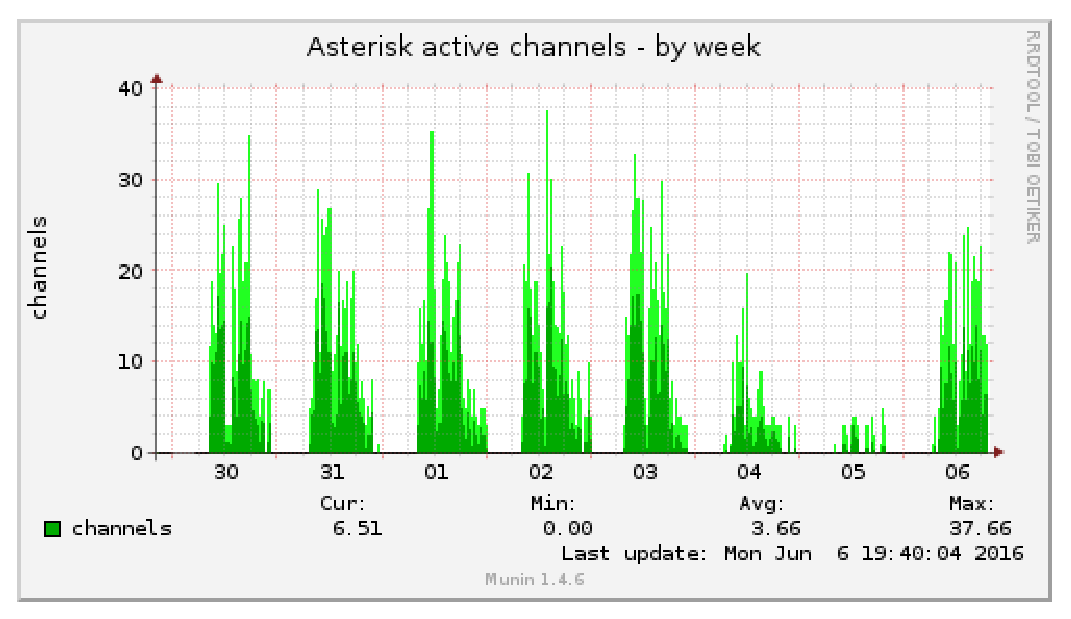
\includegraphics[width=280px]{img/simplesip_week.eps}
 \caption{Gráfico da quantidade de canais ativos simultaneamente no servidor de telefonia durante o período de uma semana.}
 \label{fig:simplesip_week}
\end{figure}

O gráfico da Figura \ref{fig:simplesip_week} mostra a quantidade de canais ativos no servidor de telefonia. Observa-se que ocorrem 
de 20 a 30 ligações simultâneas durante o horário comercial, que é das 08:00 às 12:00 e das 13:00 às 18:00. Também pode-se observar, na Figura 
\ref{fig:dns_udp} (b), que esse serviço possui um elevado número de requisições \ac{UDP}\footnote[1]{Esse número de requisições \ac{UDP} 
deve-se ao fato da telefonia utilizar o protocolo \ac{UDP} para a transmissão de voz.}, quando comparado aos demais servidores.

\section{Resumo e os serviços críticos}
\label{section:maqservcrit}

A partir da análise feita conclui-se que os servidores com maior importância para a empresa são:
\begin{itemize}
 \item \textit{Passata}: servidor de \ac{DNS} recursivo utilizado tanto pelo provedor quanto pela empresa;
 \item \textit{Speedauth}: servidor \textit{Radius} para autenticação \ac{PPPoE} dos clientes do provedor;
 \item \textit{Masterauth}: servidor \textit{Radius} para autenticação \ac{PPPoE} dos clientes do provedor;
 \item \textit{Soldi}: servidor dos sistemas gerenciais da empresa e do provedor;
 \item \textit{SimplesIP}: servidor de telefonia sobre \ac{IP} para atendimento dos clientes e comunicação interna do provedor e da empresa;
\end{itemize}

Na Tabela \ref{tab:dispservcrit}, tem-se esses servidores, seus respectivos serviços, o percentual de \textit{Uptime} e o tempo de 
\textit{Downtime} por ano. Destaca-se que o serviço de telefonia do servidor SimplesIP foi implantado em 06/2015, sendo assim foi apresentada a 
medição apenas dos últimos 6 meses de 2015.
%, por isso esse possui um \textit{Uptime} elevado.
A partir da implementação da solução de alta disponibilidade deste trabalho pretende-se atingir um \textit{Uptime} superior a 99,99\% em
todos esses serviços.

\begin{table}[h!]
\caption{Serviços críticos do ano de 2015.}
\label{tab:dispservcrit}
\begin{center}
\begin{tabular}{|l|l|l|l|}\hline
\textbf{Servidor} & \textbf{Serviço} & \textbf{Uptime} & \textbf{Downtime por ano} \\\hline
Passata & DNS recursivo & 99,913\% & 7 horas 37 minutos 30 segundos \\\hline
Speedauth & Autenticação \ac{PPPoE} & 99,755\% & 21 horas 25 minutos 50 segundos \\\hline
Masterauth & Autenticação \ac{PPPoE} & 99,475\% & 33 horas 47 minutos \\\hline
Soldi & Sistemas & 99,989\% & 59 minutos 30 segundos \\\hline
SimplesIP & Telefonia & 99,997\% & 15 minutos 10 segundos \\\hline %simplesip-ping pois asterisk nao esta correto
\end{tabular}
\end{center}
\end{table}


\section{Considerações finais}

Neste capítulo foram apresentados os serviços que foram considerados críticos, sendo que os critérios utilizados para a escolha destes foram 
criados de acordo com a análise feita nos serviços, levando em consideração a importância para a empresa, para o seu ambiente e a opinião da 
direção da empresa. Pôde-se observar que a maioria dos serviços críticos estão diretamente relacionados com o provedor, o qual possui a maior
parte dos clientes. Os serviços críticos apresentados foram o \ac{DNS} recursivo primário e a autenticação \textit{Radius}, as quais possuem
um impacto direto na navegação dos clientes do provedor. E os sistemas da empresa e do provedor juntamente com a telefonia interna, que 
são responsáveis pela gestão e pela gerência e operação da empresa e do provedor.
No próximo capítulo serão apresentadas as ferramentas escolhidas para implementação do ambiente de alta disponibilidade. 
